% !TEX encoding = UTF-8 Unicode
% VLDB template version of 2020-08-03 enhances the ACM template, version 1.7.0:
% https://www.acm.org/publications/proceedings-template
% The ACM Latex guide provides further information about the ACM template

\documentclass[sigconf, nonacm, spanish]{acmart}

%% The following content must be adapted for the final version
% paper-specific
%\newcommand\vldbdoi{XX.XX/XXX.XX}
%\newcommand\vldbpages{XXX-XXX}
% issue-specific
%\newcommand\vldbvolume{14}
%\newcommand\vldbissue{1}
\newcommand\vldbyear{2021}
% should be fine as it is
\newcommand\vldbauthors{\authors}
\newcommand\vldbtitle{\shorttitle} 
% leave empty if no availability url should be set
\newcommand\vldbavailabilityurl{https://github.com/ElenaVillano/sentiment_analysis_tweets}
% whether page numbers should be shown or not, use 'plain' for review versions, 'empty' for camera ready
\newcommand\vldbpagestyle{plain} 

%\usepackage[table,xcdraw]{xcolor}
\usepackage[spanish]{babel}
%\patchcmd{\thebibliography}{\chapter*}{\section*}{}{} % Para que la bibliografía aparezca en la misma página
\addto\captionsspanish{\renewcommand{\bibname}{Referencias}}

\newcommand{\newpara}
    {
    \vskip 0.5cm
    }


\begin{document}
\title{Análisis de sentimientos con tweets\vspace{1em}}

%% The "author" command and its associated commands are used to define the authors and their affiliations.
\begingroup
\author{Elena Villalobos}
\affiliation{%
  \institution{Instituto Tecnológico Autónomo de México}
  \city{villaele14@gmail.com}
}
\email{ }

\author{Carolina Acosta}
\orcid{0000-0002-1825-0097}
\affiliation{%
  \institution{Instituto Tecnológico Autónomo de México}
  \city{carolina.acostatovany@gmail.com}
}
\email{ }

\author{Edgar Bazo}
\orcid{0000-0001-5109-3700}
\affiliation{%
  \institution{Instituto Tecnológico Autónomo de México}
  \city{ing.edbaz@gmail.com}
}
\email{ }
\endgroup

%%
%% The abstract is a short summary of the work to be presented in the
%% article.
%\begin{abstract}https://www.overleaf.com/project/6091538289e4433ba9630d31

%\end{abstract}



%%% do not modify the following VLDB block %%
%%% VLDB block start %%%
%pagestyle{\vldbpagestyle}
%\begingroup\small\noindent\raggedright\textbf{Formato de Referencia:} Villalobos, E., Acosta, C., \& Bazo, E. (2021) \vldbtitle.\\
%\endgroup
%\begingroup
%\renewcommand\thefootnote{}\footnote{\noindent
%This work is licensed under the Creative Commons BY-NC-ND 4.0 International License. Visit \url{https://creativecommons.org/licenses/by-nc-nd/4.0/} to view a copy of this license. For any use beyond those covered by this license, obtain permission by emailing \href{mailto:info@vldb.org}{info@vldb.org}. Copyright is held by the owner/author(s). Publication rights licensed to the VLDB Endowment. \\
%\raggedright Proceedings of the VLDB Endowment, Vol. %\vldbvolume, No. \vldbissue\ %
%ISSN 2150-8097. \\
%\href{https://doi.org/\vldbdoi}{doi:\vldbdoi} \\
%}\addtocounter{footnote}{-1}\endgroup
%%% VLDB block end %%%

%%% do not modify the following VLDB block %%
%%% VLDB block start %%%

%%% VLDB block end %%%

\maketitle
\section*{RESUMEN}

Una de las redes sociales más utilizadas para interactuar socialmente es la plataforma de \textit{Twitter}. El objetivo del presente trabajo es analizar el texto contenido en \textit{tweets} y construir una red neuronal que clasifique si el sentimiento del mismo es positivo o negativo. Se utilizó una base de datos que contiene 1.6 millones de \textit{tweets}, con su respectiva clasificación. El modelo de redes neuronales creado se basó en el campo de estudio de Procesamiento de Lenguaje Natural. Se encontró un modelo que nos da resultados relativamente buenos, generando una clasificación adecuada del contenido de los \textit{tweets}. Dicho modelo utiliza capas de \textit{embedding} al inicio, redes de memoria a corto plazo y pocas capas ocultas.

\vspace*{0.5em}

\begingroup\small\noindent\raggedright\textbf{Formato de Referencia:} Villalobos, E., Acosta, C., \& Bazo, E. (2021). Análisis de sentimientos con tweets.\\
\endgroup

\ifdefempty{\vldbavailabilityurl}{}{
\begingroup\small\noindent\raggedright\textbf{Disponibilidad de artefactos:} El código fuente, los notebooks de trabajo, y otros recursos para llevar a cabo este proyecto están disponibles en: \url{\vldbavailabilityurl}.\\
\endgroup
}

\ifdefempty{\vldbavailabilityurl}{}{
\begingroup\small\noindent\raggedright\textbf{Palabras clave:} Aprendizaje profundo, análisis de sentimientos, minería de texto, LSTM, redes neuronales, Python, redes sociales, Twitter.
\endgroup
}

\section{Introducción}

%Un párrafo explicando el problema que vamos a enfrentar.
Hoy en día, las redes sociales son un medio de comunicación muy utilizado para conocer las opiniones actuales sobre diversos temas. Una primera aproximación para conocer y/o describir los procesos de comunicación en estas redes, es saber si los comentarios u opiniones tienen alguna connotación positiva o negativa. Una de las redes sociales más utilizadas para monitorear la conversación pública es \textit{Twitter}; por lo que, nos vamos a enfocar a estudiar dicha red social. Específicamente, el objetivo del presente proyecto es analizar el contenido de \textit{tweets} y poder construir un clasificador que aprenda a distinguir entre una opinión positiva o negativa.

%Uno o dos párrafos(puede ser subsección) explicando los datos(fuente, tamaño de la bd, no. de variables, formato de entrada x y salida y, hay outliers? , divisón entrenamiento, validación y prueba.
Los datos que utilizaremos fueron recolectados de \textit{Twitter}, por la empresa H20 \cite{H20}, acerca del Huracán Harvey que tenían como intención identificar \textit{tweets} con diferente connotación de sentimientos. El conjunto de datos tiene las siguientes características:
\begin{itemize}
\item Idioma: Inglés.
\item Observaciones: 1.6 millones.
\item Variables: 
    \begin{itemize}
    \item \textbf{\texttt{target:}} Polaridad del tweet, positivo o negativo. 
    \item \texttt{ids:} ID tweet.
    \item \texttt{date:} Fecha y hora del tweet.
    \item \texttt{flag:} Si hubo algún tipo de \textit{query}.
    \item \texttt{user:} Usuario del tweet
    \item \textbf{\texttt{text:}}Texto del tweet
    \end{itemize}
\end{itemize}

La variable que utilizamos para entrenar es \texttt{text}, que contiene sólo el \textit{tweet} sin \textit{emojis}; y la variable que utilizamos como etiqueta es la \texttt{target}.

\subsection{Procesamiento de Lenguaje Natural (NLP)}
%Mencionar brevemente qué tipo de modelo usan para atacar el problema
En este proyecto construimos un modelo con base en Procesamiento de Lenguaje Natural (NLP, por sus siglas en inglés) para realizar el análisis de sentimientos. El Procesamiento del Lenguaje Natural es el campo de estudio que se enfoca en la comprensión del lenguaje humano mediante una computadora, siendo así una rama de aprendizaje profundo \cite{notas_clase}.

\section{Trabajos relacionados}

%Comentar brevemente algunos trabajos que puedan leer, y que hayan hecho algo similar, al menos 3 trabajos. 

%Un párrafo por trabajo, qué datos usaron, y qué problemas partirucalres reportan, qué modelo usaron, cómo es la calidad de su solución.

Jacob, en \textit{StreamHacker} \cite{Jacob}, describe que se enfocó en la clasificación de sentimientos positivos o negativos. Utilizó datos del paquete \textit{NLTK} para el corpus de \textit{reviews} de películas. Empezó utilizando un simple clasificador de \textit{Naive Bayes} como base, y extrajo las variables de forma booleana. Con poca manipulación de los datos logró obtener una exactitud del 73\%, lo cual es cerca de la exactitud humana; se dice que los humanos concuerdan en sentimientos sólo el 80\% del tiempo.

El objetivo del proyecto que realizó Laurent Luce \cite{Laurent} es clasificar un \textit{tweet} positivo o negativo. Utilizó datos que extrajo manualmente, y fueron alrededor de 600 \textit{tweets} positivos y 600 \textit{tweets} negativos para el entrenamiento del clasificador. Utilizó \textit{tweets} sin \textit{hashtags}, sin menciones ni \textit{emojis}. La única imputación que realizó fue eliminar las palabras menores de 2 letras y tener todo en minúsculas. Para crear el clasificador, primero se hizo una extracción de variables para saber cuáles eran las variables relevantes; y el clasificador utilizado fue \textit{Naives Bayes} de \textit{NLTK}. Con sus datos de prueba logró un 80\% de exactitud.

La empresa que desarrolla H20 \cite{H20}, realizó un proyecto donde el objetivo fue extraer \textit{tweets} relevantes para el caso del huracán Harvey, utilizando el conjunto de datos de \texttt{'sentiment140'} que ya se encuentran etiquetados como sentimientos positivos o negativos, y así construir un clasificador que aprenda a diferenciar entre un \textit{tweet} negativo o serio y un \textit{tweet} positivo. El siguiente objetivo fue utilizar este clasificador para \textit{rankear} los \textit{tweets} basados en un porcentaje de severidad y así poder extraer el \textit{top} de \textit{tweets} que necesiten ayuda en la situación actual, en este caso, el huracán Harvey o Irma. Para la transformación de sus datos utilizaron TF-IDF, éste extrae para cada palabra qué tan importante es para ese \textit{tweet}. Después de la transformación, utilizaron \textit{H20 Gradient Boosting} para entrenar y obtener que el clasificador logré diferenciar entre un \textit{tweet} positivo o negativo. No indican cuál es el porcentaje de su exactitud obtenida.

\section{Análisis exploratorio}

Se realizó un análisis exploratorio de las variables \texttt{target} y \texttt{text}. La primera variable está balanceada; es decir, contiene el 50\% de observaciones positivas y 50\% negativas. Los valores que venían por defecto eran 4 para la asignación positiva y 0 para la asignación negativa. En cuando a la segunda variable, \texttt{text}, se muestran gráficos de nubes de palabras, en los cuales el tamaño de la palabra está relacionado a su frecuencia. La figura \ref{fig:neg} muestra los \textit{tweets} con etiquetas negativas, y las palabras que más resaltan son: \textit{day, rest, text, aww, bummer, shoulda}. La figura \ref{fig:pos} tiene los tweets con etiquetas positivas, donde las palabras que más resaltan son: \textit{meet, best, happi, besti, guy, tonight}. Es importante mencionar que para ambos gráficos de nubes de palabras, se realizó un pre-procesamiento de limpieza, descrito a continuación. 


\begin{figure}
  \centering
  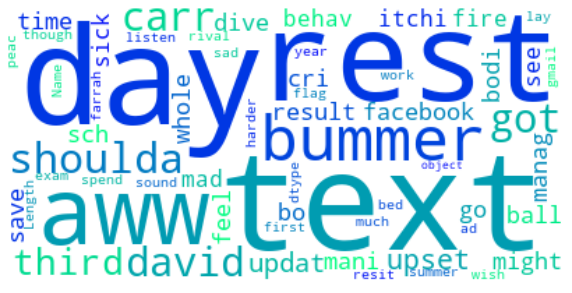
\includegraphics[width=\linewidth]{figures/wordcloud_negativo}
  \caption{Nube de palabras con etiquetas negativas.}
  \label{fig:neg}
\end{figure}

\begin{figure}
  \centering
  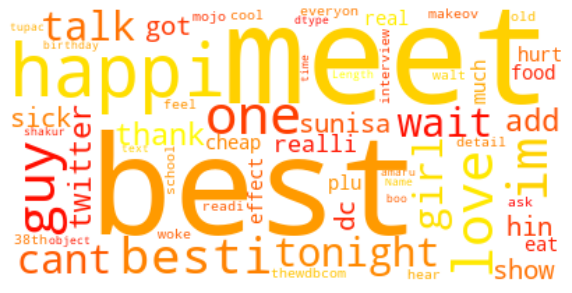
\includegraphics[width=\linewidth]{figures/wordcloud_positivo}
  \caption{Nube de palabras con etiquetas positivas.}
  \label{fig:pos}
\end{figure}

\section{Solución}
\subsection{Limpieza de datos}
%Primero explicar cualquier preprocesamiento que hayan hecho sobre los datos. 
Antes de realizar cualquier tarea de Procesamiento de Lenguaje Natural es importante que nuestros datos tengan cierto grado de limpieza. En el Cuadro \ref{tab:commands}. mostramos ejemplos de textos procesados por nuestro algoritmo que contiene las siguientes tareas de limpieza:

\begin{enumerate}
\item Convertir todo el texto a minúsculas.
\item Quitar:
\begin{enumerate}
    \item Caracteres codificados en html (\&amp;, \&quot;, \&lt;, \&gt;).
    \item URLs, menciones a usuarios y RT.
    \item \# y mantener sólo la palabra o conjunto de palabras.
    \item Espacios o puntos extras.
    \item Caracteres especiales (’"?!,.():;-).
    \item Letras repetidas (\textit{sooooo haaappy}).
    \item Caracteres ascii y Descifrar a utf-8.
\end{enumerate}
\item Separar abreviaciones.
\item Quitar \textit{stopwords}.
\item Realizar \textit{stemming} y lematización.
\item Modificar etiquetas (0 = negativo, 1 = positivo).

\end{enumerate}



\begin{table*}[t]
  \caption{Ejemplo de limpieza de texto}
  \label{tab:commands}
  \begin{tabular}{|c|c|}
    \toprule
    Texto original & Texto limpio \\
    \midrule
    \vtop{\hbox{\strut @switchfoot http://twitpic.com/2y1zl - awww, that's a bummer.}\hbox{\strut you shoulda got david carr of third day to do it. ;d }}
    & aww bummer shoulda got david carr third day  \\
    \hline
    @RunningGolfer Glad you picked it up...she didn't &  lad pick upsh   \\
    \hline
    @i140 I'm excited I made it on your list.  Thnx, Jason. &  excit made list thnx jason   \\
    \hline
    \vtop{\hbox{\strut @johncmayer Where is that Belgian concert you were}\hbox{\strut talking about? I can't even find it on google  }}
    & belgian concert talk even find googl  \\
    \hline
    \vtop{\hbox{\strut sitting on a field with Emma and Miri watching Sarah and }\hbox{\strut Naomi running around searchinf for elves }}
    & 
    \vtop{\hbox{\strut sit field emma miri watch sarah  }\hbox{\strut naomi run around searchinf elv  }}  \\
    \hline
    \vtop{\hbox{\strut Couldn't decide if I wanted to go to Family Fortunes on Sunday  }\hbox{\strut but train is  £45 now   Its the Christmas special being filmed on that day!! }}
    & 
    \vtop{\hbox{\strut could decid want go famili fortun sunday  }\hbox{\strut train 45 christma special film day  }}  \\
    
    \bottomrule
  \end{tabular}
\end{table*}

Para quitar texto o ciertos caracteres de nuestro texto, utilizamos expresiones regulares, que a continuación presentamos cada una de ellas.

\subsubsection{Caracteres HTML}

En los \textit{tweets} encontramos caracteres con código HTML que se utilizan con frecuencia, como: \&, ``, < y >. Cada uno tiene su código en HTML representado por: ``\&amp'', ``\&quot;'', ``\&lt;'' y ``\&gt;'', respectivamente. Y su expresión regular es exactamente el código representado.

\subsubsection{URLs}

Las \textit{Uniform Resource Locator}, (URL por sus siglas en inglés), son utilizadas en los \textit{tweets} de manera frecuente para indicar la liga a una página web. La expresión regular que corresponde es \verb$((www\.[\S]+)|(https?://[\S]+))$.

\subsubsection{Menciones a usuarios}

Es común que los usuarios mencionen a otros usuarios, y ésto se realiza con el caracter @. La expresión regular asociada a identificar las menciones es \verb$@[\S]+$.

\subsubsection{Retweets}

Los \textit{Retweets} son publicaciones duplicadas desde otro usuario y para identificarlas con expresiones regulares utilizamos \verb${\brt\b}$.

\subsubsection{Hasthags}

El procesamiento de los \textit{hashtags}, es simplemente eliminar el caracter \# y quedarnos con la palabra. Para identificar un \textit{hasthag} con expresiones regulares utilizamos \verb$#(\S)+$.

\subsubsection{Letras repetidas}

Es común que los usuarios expresen sus sentimientos repitiendo letras como \textit{``I'm sooooo haaaapppyyyy''}, lo cual es variable entre usuarios. Decidimos reducir la repetición a lo máximo dos letras repetidas por letra, ya que en el idioma inglés es común tener letras repetidas en las palabras como \textit{``happy''}. De igual forma, utilizamos expresiones regulares para identificar estos casos y su correspondiente es \verb$(.)\ 1+', r'\ 1\ 1$.

\subsubsection{Stopwords}

Para nuestra limpieza también removemos las palabras vacías o \textit{stopwords}, que en el lenguaje humano ayudan en la lógica de las oraciones pero no tienen significado en el procesamiento de lenguaje natural, como lo son, los artículos, pronombres, preposiciones, etc. Las \textit{stopwords} las obtenemos de la paquetería \textit{NLTK} \cite{nltk}, utilizando el idioma inglés.

\subsubsection{Stemming y lematización}

Se refiere a eliminar sufijos morfológicos a una palabra; es decir, reducir la palabra a un ``lema''; por ejemplo, \textit{mention}, \textit{mentioning}, \textit{mentioned} son palabras que su lema llega a ser \textit{ment}. Para realizar este proceso utilizamos la paquetería de \textit{NLTK} \cite{nltk}, el tokenizador \texttt{word\_tokenizer} y el \textit{stem} \texttt{PorterStemmer}. 

\subsubsection{Modificación de etiquetas}

Los datos originales contienen una variable \texttt{target} que tomamos como etiqueta, y los valores toma son ``0'' o ``4'' si son negativos o positivos, respectivamente. Para nuestro problema decidimos cambiarlo a ``0'' y ``1'' para negativos y positivos, respectivamente; ya que la distancia entre 0 y 1 es más corta que 0 y 4 para un clasificador.

\subsection{Tokenizador}

Posteriormente a la limpieza de texto, nos enfocamos en hacer otro tipo de pre-procesamiento al texto utilizando un Tokenizador, que se encarga de vectorizar el texto. Es decir, convierte cada palabra en una secuencia de enteros; nosotros utilizamos el Tokenizador de \texttt{Tensorflow} \cite{tersopreprocessing}. 

Una vez realizado el proceso de tokenización, obtenemos 330,671 palabras en nuestro diccionario, y para determinar el tamaño máximo de nuestro vocabulario, exploramos la frecuencia de cada palabra (ver figura \ref{fig:vocabulario}). Seleccionamos aquellas que tuvieran una frecuencia arriba de 1,500, ya que no es necesario agregar palabras a nuestro diccionario que son poco utilizadas por los usuarios. El tamaño final de nuestro vocabulario fue de 1,000 palabras.


\begin{figure}
  \centering
  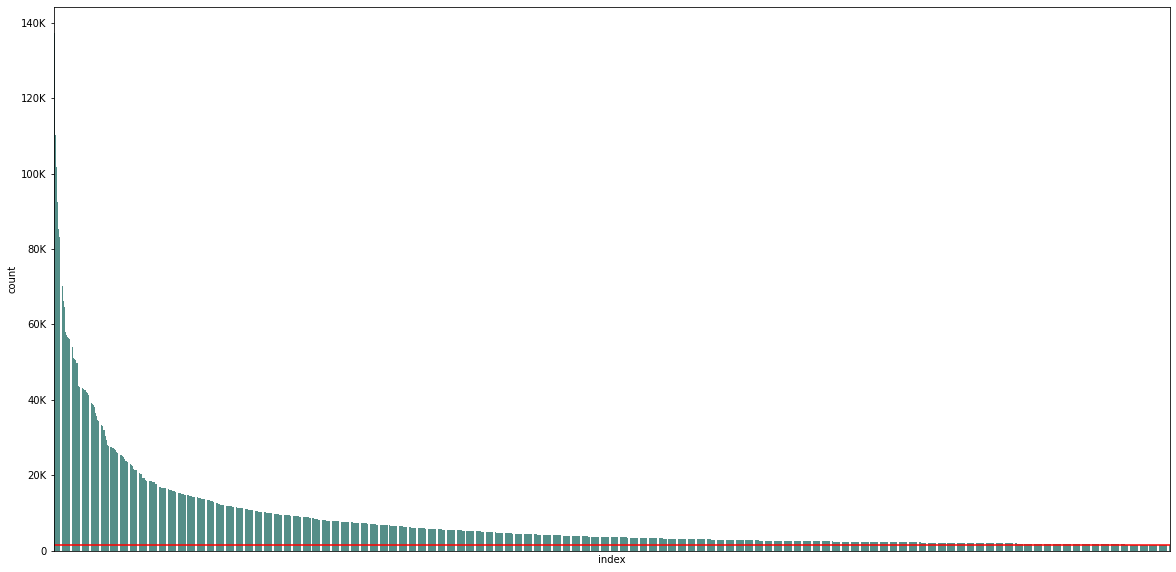
\includegraphics[width=\linewidth]{figures/1000vocabulario}
  \caption{1K palabras y su frecuencia en nuestro corpus.}
  \label{fig:vocabulario}
\end{figure}

Después de obtener el tokenizador con nuestro vocabulario, analizamos la cantidad de tokens que tiene cada oración, (ver figura \ref{fig:histogram}), y obtuvimos la cantidad máxima de tokens que se encuentra en nuestro cuantil al 95\%, que resultó ser de 11 tokens. En otras palabras, el 95\% de nuestros datos tienen 11 tokens o menos. 

Entonces, seleccionamos 11 como número máximo de tokens por oración y realizamos un \textit{padding post}, que se refiere a transformar cada secuencia de tokens al mismo tamaño, rellenando el vector al final con ceros para los datos que tenían menos de 11 tokens. El 5\% restante de los datos, no se tomó en cuenta para el modelado. De igual forma utilizamos \texttt{Tensorflow} \cite{tersopreprocessing} para realizar este procesamiento.

\begin{figure}
  \centering
  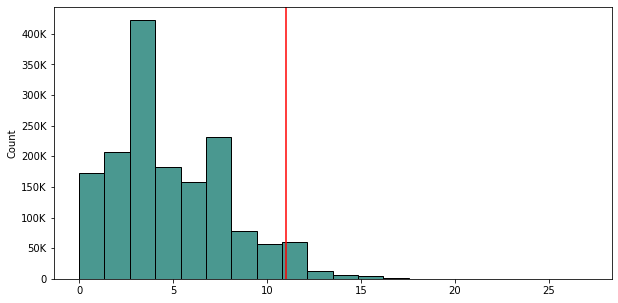
\includegraphics[width=\linewidth]{figures/histogram}
  \caption{Histograma de número de palabras por oración}
  \label{fig:histogram}
\end{figure}

\subsection{Arquitectura de la red neuronal}

La arquitectura de la red neuronal utilizada se observa en la figura \ref{fig:architecture}. El modelo consta de 4 capas, la primera siendo de entrada y \textit{Embedding}. La segunda es una capa bidireccional \textit{LSTM} con 12 unidades y un \textit{dropout} de 0.5. Las siguiente capa oculta esta formada por 24 neuronas estándar con un \textit{dropout} de 0.5 y una función de activación \textit{ReLu}. Por último, la capa de salida consta de una neurona con función de activación sigmoide.


\begin{figure}
  \centering
  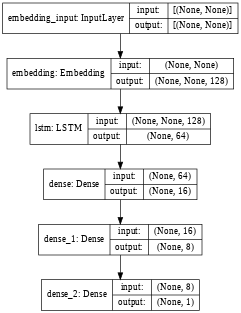
\includegraphics[width=\linewidth]{figures/arquitectura}
  \caption{Extracción del diagrama de nuestro modelo en \textit{Tensorflow.Keras}}
  \label{fig:architecture}
\end{figure}

\subsubsection{Capa Embedding} 

Esta capa se utiliza al principio de la red neuronal debido a que realiza específicamente un procesamiento de texto que asigna un significado similar a la representación numérica de las palabras; en otras palabras, toma en cuenta el contexto relativo de las palabras para representarlas en un espacio numérico. Como parámetros de entrada especificamos el tamaño del vocabulario, la dimensión de nuestra salida y la longitud de las secuencias \cite{notas_clase, embedding, embedding2}.


\subsubsection{Red Long Short Term Memory}

Que hace referencia a una red neuronal recurrente (i.e. \textit{RNN}) de memoria a corto plazo (\textit{LSTM} por sus siglas en inglés). Esta capa permite retroalimentación entre neuronas y procesa secuencias en los datos, por lo que puede recordar información previa para decidir los siguientes estados. Esto es muy útil para el procesamiento de texto, pues el lenguaje natural utiliza una estructura similar. Además, esta red soluciona el problema de perder cohesión cuando la red no es capaz de conectar entre dependencias, que sucede cuando las entradas de datos son muy grandes; por lo que funciona como buena alternativa a las \textit{RNN} \cite{notas_clase, lstm, lstm_use}.

\subsubsection{Capa bidireccional}

Esta es una extensión de la red neuronal recurrente de memoria a corto plazo, que de acuerdo a algunas referencias \cite{notas_clase, bidireccional, bidi2}, puede mejorar el desempeño del modelo en problemas secuenciales de clasificación, tal como la estructura de nuestro conjunto de datos. 

\subsubsection{Funciones de activación y modelo}

Es común que en la práctica se utilice la función de activación \textit{ReLU} para capas ocultas \cite{notas_clase}, debido a que permite a la red neuronal aprender dependencias no lineales. 

\begin{equation}
  f(x) = max (0,x) =  \left \{ \begin{matrix} 0 & \mbox{si x<0}
\\ x & \mbox{si x>=0}\end{matrix}\right. 
\end{equation} 

Se consideró la función sigmoide como función de activación para la capa de salida, ya que nuestro problema a resolver consta de una clasificación binaria; 0 si es negativo y 1 si es positivo.

\begin{equation}
  f(x) =\frac{1}{1-\exp^{-x}}
\end{equation} 


\subsubsection{Configuración del modelo}

\begin{itemize}
    \item Optimizador: RMSprop,
\end{itemize}    
\begin{equation}
  C = C +d \cdot C \cdot (1-d) \cdot \Delta W^2
\end{equation}  

\begin{equation}
  W = W - \frac{\alpha \cdot \Delta W}{\sqrt{C + \epsilon}}
\end{equation} 
    
%\begin{equation}
%  c = \beta_1 \cdot m + (1 - \beta_1) \cdot \Delta W
%\end{equation} 

%\begin{equation}
%  v = \beta_2 \cdot v + (1 - \beta_2) \cdot \Delta W^2
%\end{equation} 

%\begin{equation}
%  W = W - \frac{\alpha \cdot \Delta W}{\sqrt{C + \epsilon}}
%\end{equation} 

\begin{itemize}
    \item Función de pérdida: Binary Cross Entropy,
\end{itemize}    

\begin{equation}
%l_{BCE} = -(y\log_2(\hat y) + (1 - y) \log_2(1-\hat y)),
H_q(q) = - \frac{1}{n} \sum_{i=1}^n y_i \cdot log(p(y_i)) + (1 - y_i) \cdot log(1-p(y_i))
\end{equation}

donde $y$ es la etiqueta y $p(y)$ la probabilidad de que la predicción sea 1.

\begin{itemize}
    \item Métricas: Binary accuracy y accuracy.
\end{itemize}


\subsubsection{Ajuste del modelo}
\begin{itemize}
    \item Épocas: 20.
    \item Tamaño de lote: 64.
    \item Tamaño de conjunto de validación: 20\%.
\end{itemize}

Después de la limpieza de texto a nuestros 1.6 millones de datos, obtuvimos 1,591,506 que realmente tenían contenido y éstos los separamos en 70\% para entrenar y 30\% para pruebas. Por lo tanto, para entrenar utilizamos 1,114,054 datos de los cuales 20\% se asignaron para validación.

\subsection{Comparaciones de modelos}

En el presente proyecto experimentamos con alrededor de 30 modelos con diversas configuraciones e hiper-parámetros. El modelo que mejor se ajustó y predijo mejor los datos fue el presentado en la figura \ref{fig:architecture}. Sin embargo, a continuación presentaremos algunas de las configuraciones probadas más relevantes y diversas reflexiones sobre el uso de las mismas. 

\begin{itemize}

\item Tamaño de datos: En las primeras iteraciones probamos evaluar los modelos con datos de entre 50K y 200K para reducir el tiempo de cómputo, en dichas iteraciones salieron precisiones de alrededor del 70\%. Al utilizar los 1.6 millones aumentó la precisión en 5 puntos porcentuales, por lo que elegimos trabajar con la base completa.

\item Cantidad de palabras: Encontramos que utilizar un número mayor de palabras (10K) mejoraba mucho el ajuste del modelo. Sin embargo, esto a su vez hace que tengamos muchas palabras con frecuencia muy baja, por lo que al final la predicción de estos modelos no era tan buena. Los modelos que tenían menor número de palabras predecían mejor los sentimientos de los \textit{tweets}. Debido a esto, utilizamos 1,000 palabras, de las 330,671 generadas en el diccionario de tokens (ver figura \ref{fig:vocabulario}). 

\item Longitud de la secuencia: Cada \textit{tweet} se convierte en un vector de enteros (secuencia) que depende de su mismo número de palabras, probamos modelos con diferente secuencia y encontramos que utilizar la longitud de 11, mejoraba también el desempeño del modelo (ver figura \ref{fig:histogram}). 

\item \textit{Padding}: El relleno de las secuencias se puede realizar al inicio o al final, observamos que hacerlo al final era mejor que hacerlo al inicio.

\item Número de capas: Debido a que estamos utilizando capas recurrentes, no es necesario colocar demasiadas capas para el modelo, por lo que en general probamos modelos con capas de no más de 8.

\item Número de unidades en capas: Para este hiper-parámetro utilizamos unidades de 8, 12, 24 o 64; las unidades que mejor funcionaron fueron 12 y 24. 

\item Función de activación: El desempeño fue muy similar entre los optimizadores RMSprop y Adam, al final, se decidió mantener el optimizador RMSprop.

\item Capa bidireccional: El uso de esta capa no se observó que fuera determinante para mejorar el desempeño de los modelos en general. Sin embargo, resultó ser parte del modelo final elegido.

\item\textit{Dropouts}: Existieron algunas evaluaciones en los modelos donde la precisión del conjunto de validación era más alto que la precisión del conjunto de entrenamiento. Se encontró que esto se puede deber a varias razones \cite{notas_clase,sanity,over_fittin}, una de ellas es el uso de la técnica de regularización \textit{dropout} en la red, que oculta temporalmente neuronas de la red en el conjunto de entrenamiento, pero no necesariamente en el conjunto de validación. A consecuencia de esto, realizamos iteraciones donde se quitó esta técnica y se encontró que efectivamente, ya no generaba el problema de que la precisión en el conjunto de validación era más grande que en el de entrenamiento. 

\end{itemize}

\section{Resultados}

Las métricas en los diferentes conjuntos de entrenamientos se pueden observar en el Cuadro \ref{tab:resultados}. En ésta se observa que no hay una diferencia muy grande entre los conjuntos de datos, tanto para la precisión como para la pérdida. 

\begin{table}[ht]
  \caption{Resultados obtenidos en entrenamiento, validación y prueba}
  \begin{tabular}{|c|c|c|c|}
    \toprule
      & \textbf{Entrenamiento} & \textbf{Validación} & \textbf{Prueba} \\
    \midrule
    
    \textbf{Precisión} & 75.09\% & 74.97\% & 75.18\% \\
    \hline
    \textbf{Pérdida} & 0.5236 & 0.5118 & 0.5102 \\
    \bottomrule
  \end{tabular}

 \label{tab:resultados}
\end{table}


La figura \ref{fig:loss} se muestra la pérdida del modelo, a través de las épocas, para el conjunto de entrenamiento y el de validación. Se observa que en las primeras épocas la pérdida para el conjunto de entrenamiento (línea azul) disminuye en varias unidades, sin embargo, a partir de la época 8 parece incrementar unas cuántas unidades. En cuanto al conjunto de validación (línea naranja), se mantiene a lo largo de todas las épocas por debajo del conjunto de entrenamiento, y parece tener un comportamiento consistente, excepto por el pico observado en alguna de las últimas épocas.

La figura \ref{fig:accuracy} muestra la precisión del modelo a lo largo de las épocas para el conjunto de entrenamiento (línea azul) y el de validación (línea naranja). La precisión de entrenamiento sobrepasa el 75.2\% durante algunas épocas intermedias y la precisión de validación oscila entre 74.9\% y 75\%. La línea naranja siempre se observa por debajo de la azul, y ambas tienen un comportamiento similar; que puede ser un indicador de que nuestro modelo no tiene algún tipo de sobre-entrenamiento o sub-entrenamiento.

\begin{figure}
  \centering
  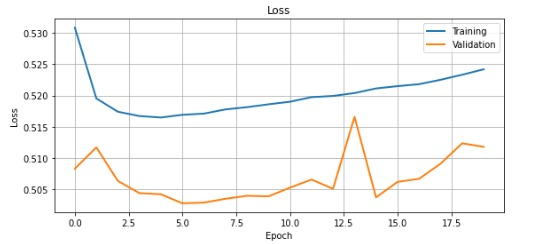
\includegraphics[width=\linewidth]{figures/loss}
  \caption{Pérdida del modelo a lo largo de las épocas.}
  \label{fig:loss}
\end{figure}

\begin{figure}
  \centering
  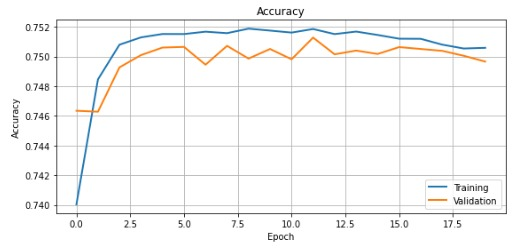
\includegraphics[width=\linewidth]{figures/accuracy}
  \caption{Precisión del modelo a lo largo de las épocas.}
  \label{fig:accuracy}
\end{figure}

Además de tener un conjunto de prueba proveniente de la base de 1.6 millones de observaciones. Obtuvimos una base que tenía 359 \textit{tweets} seleccionados, junto con su etiqueta. Decidimos evaluar la precisión de nuestro modelo con este nuevo conjunto de datos, para analizar de manera más detallada el comportamiento de nuestro modelo. A dicho conjunto, le aplicamos la misma limpieza de datos ya presentada anteriormente y mostramos tres ejemplos en el Cuadro \ref{tab:predicciones}. En este cuadro, observamos tres ejemplos, dos donde el modelo acierta correctamente y uno en el que no. Este último parece tener un poco más de ambigüedad que los predichos correctamente, lo cual puede ser la razón por la cuál el modelo se equivocó en predecir dicho texto.


\begin{table*}[t]
  \caption{Ejemplo predicciones en la base de prueba adicional.}
  \label{tab:predicciones}
    \begin{tabular}{|c|c|c|c|}
    \toprule
Texto original & Texto pre-procesado & Etiqueta real & Etiqueta predicha \\
\hline
how can you not love Obama? he makes jokes about himself. & love obama make joke & Positive      & Positive \\
\hline
cant sleep... my tooth is aching. & cant sleep tooth ach & Negative & Negative \\
\hline

    \vtop{\hbox{\strut I just created my first LaTeX file from scratch. That didn't work}\hbox{\strut out very well. (See @amandabittner , it's a great time waster)  }}
  & 
    \vtop{\hbox{\strut creat first latex file scratch work }\hbox{\strut well see great time waster)  }}
   & Negative      & Positive  \\
   \bottomrule
    \end{tabular}
\end{table*}

Asimismo en cuanto a las métricas obtenidas en este nuevo conjunto de datos, la precisión obtenida fue del 76.6\%, teniendo 84 \textit{tweets} clasificados erróneamente. 

\subsection{Análisis de desempeño obtenido y problemas encontrados}

La razón por la que se pudo obtener un desempeño ``relativamente bueno'' recae en diversas razones, una de ellas siendo el uso de pocas capas ocultas y una recurrente con memoria a corto plazo. Como se mencionó anteriormente, una capa recurrente permite retroalimentación entre neuronas y procesa la secuencia que esperamos obtener tomando en cuenta el contexto del texto, que es muy útil para la naturaleza de nuestros datos.

Uno de los problemas encontrados se relaciona con el \textit{tweet}, hay ciertos usuarios que utilizan muchas letras repetidas para expresar sus opiniones y lo que logramos fue reducirlo a dos palabras repetidas, pero nunca a la palabra original. De igual forma, buscar una base que tenga el texto completamente limpio, sin faltas de ortografía o con completa coherencia, es difícil de alcanzar por la cantidad de palabras y todas las posibles variaciones que usamos los seres humanos al comunicarnos con texto; sobre todo teniendo la libertad de escritura que proporciona la plataforma de \textit{Twitter}. 

A pesar de lo anterior, consideramos que una de las posibles razones por la cual obtuvimos resultados relativamente buenos, fue la limpieza del texto. Esto ayudó a generalizar la forma de las palabras en sus diferentes tiempos, quitar palabras sin sentido para el análisis, y quitar fuentes de ruido que pueden afectar la estimación del modelo. Al final, todo esta limpieza generó una reducción en el tamaño del vocabulario y que la frecuencia aumentara para cada una de las secuencias. 

Otro problema encontrado fue que a pesar de probar de diferentes configuraciones de hiper-parámetros, hacer un pre-procesamiento de texto detallado, utilizar secuencias de tokens asociadas al tamaño de los \textit{tweets}, e incluso hacer uso de diferentes números y tipos de capas, ningún modelo pudo subir su precisión a más de 75\%. Creemos que esto se puede deber a la base de datos o a la misma característica del lenguaje que tiende a ser muy complejo. 

\section{Conclusiones}

Uno de los principales logros del presente trabajo fue obtener un modelo relativamente bueno y adecuado que obtuvo buenas métricas a través de los diferentes conjuntos de datos, e incluso con un conjunto de datos de prueba adicional. Esto se podría considerar un buen aproximado a lo que un humano puede predecir cuando se le pide que categorice sentimientos positivos o negativos, que éste califica correctamente los sentimientos con un 80\% de precisión, como lo menciona el artículo de Jacob en StreamHacker \cite{Jacob}. 

Un logro adicional, fue el aprendizaje del comportamiento de modelos de redes neuronales profundas enfocados a evaluar lenguaje. Si bien, la complejidad de la estructura en la comunicación escrita puede ser muy grande, estos modelos nos presentan una buena aproximación a segmentar dicha complejidad y estudiar partes específicas de la misma para ir generando mayor conocimiento en el área.

Además, la limpieza y descripción de estos \textit{tweets}, nos mostró que a pesar de tener una gran variedad de palabras en el idioma inglés, realmente no se utiliza mucha de esta riqueza para expresar sentimientos positivos y/o negativos. Lo cual no es algo malo necesariamente, pues habla de que estos sentimientos pueden ser más sencillos de lo que realmente pensamos. Sin embargo, una siguiente aproximación a este problema podría ser agregar una categoría neutral, pues no necesariamente todos los textos entran sólo en estas dos categorías, y muchas veces tienen una intención de informar más allá de expresar un sentimiento.

En este proyecto el procesamiento de todos los modelos evaluados se utilizaron unigramas (una palabra completa como token) del texto por lo que se podría sugerir que en futuras investigaciones se utilice bigramas (dos palabras como token) pensado como una posible mejora para el modelo. 

Finalmente, el presente proyecto se realizó con \textit{tweets} en el idioma inglés, por lo que un camino muy adecuado sería probar este tipo de modelos en el idioma de español. Además, se podrían buscar \textit{tweets} referentes a un sólo tema, como elegir un \textit{hashtag} específico o un acontecimiento social en cierto periodo tiempo, para ayudar al estudio del Procesamiento de Lenguaje Natural.





%\begin{acks}
% This work was supported by the [...] Research Fund of [...] (Number [...]). Additional funding was provided by [...] and [...]. We also thank [...] for contributing [...].
%\end{acks}

%\clearpage

\begin{thebibliography}{3}

\bibitem{H20}
\textit{Social Machine Learning with H20, Twitter, Python.}
[\url{https://www.linkedin.com/pulse/social-machine-learning-h2o-twitter-python-marios-michailidis/}].

\bibitem{Jacob}
\textit{Jacob, 2010. StreamHacker. Text classification for sentiment analysis - Naive Bayes Classifier.}
[\url{https://streamhacker.com/2010/05/10/text-classification-sentiment-analysis-naive-bayes-classifier/}].

\bibitem{Laurent}
\textit{Laurent Luce, 2012. LaurentLuce. Twitter sentiment analysis using Python and NLTK.}
[\url{http://www.laurentluce.com/posts/twitter-sentiment-analysis-using-python-and-nltk/}].

\bibitem{notas_clase}
\textit{Notas del curso de Aprendizaje profundo con el profesor Edgar Roman-Rangel.}

\bibitem{nltk}
\textit{Documentación NLTK}
[\url{https://www.nltk.org/}].

\bibitem{tersopreprocessing}
\textit{Documentación Tensorflow, keras, pre-procesamiento.}
[\url{https://www.tensorflow.org/guide/keras/preprocessing_layers}].

\bibitem{embedding}
\textit{Documentación Keras embedding.}
[\url{https://keras.io/api/layers/core_layers/embedding/}].

\bibitem{embedding2}
\textit{How to use word Embedding Layers for Deep learning with Keras.}
[\url{https://machinelearningmastery.com/use-word-embedding-layers-deep-learning-keras/}].

\bibitem{lstm}
\textit{Documentación keras LSTM layer.}
[\url{https://keras.io/api/layers/recurrent_layers/lstm/}].


\bibitem{lstm_use}
\textit{Implementation of LSTM layers.}
[\url{https://towardsdatascience.com/understanding-lstm-and-its-quick-implementation-in-keras-for-sentiment-analysis-af410fd85b47}].

\bibitem{bidi2}
\textit{Documentación keras de bidirectional layer.}
[\url{https://keras.io/api/layers/recurrent_layers/bidirectional/}].

\bibitem{bidireccional}
\textit{How to Develop a Bidirectional LSTM for Sequence Classification in Python with Keras.}
[\url{https://machinelearningmastery.com/develop-bidirectional-lstm-sequence-classification-python-keras}].

\bibitem{sanity}
\textit{Redes Neuronales, ``Sanity checks''.}
[\url{https://cs231n.github.io/neural-networks-3/#sanitycheck}].

\bibitem{dropout}
\textit{Documentación Tersonflow layers dropout.}
[\url{https://www.tensorflow.org/api_docs/python/tf/keras/layers/Dropout}].

\bibitem{over_fittin}
\textit{What is Dropout?}
[\url{https://www.machinecurve.com/index.php/2019/12/16/what-is-dropout-reduce-overfitting-in-your-neural-networks/}].

\end{thebibliography}
\end{document}
\endinput
